\documentclass[10pt]{article}
\usepackage[letterpaper,margin=1in]{geometry}
\usepackage{amsmath,booktabs,graphicx,array,caption,float}
\usepackage[hidelinks]{hyperref}
\usepackage{enumitem,adjustbox}
\captionsetup{font=small}
\setlist{itemsep=1pt,topsep=3pt}
\graphicspath{{./}{figs/}{images/}{figures/}{Figures/}}
\title{Project ABEONA Crew Capsule Main Engine:\\Thrust Chamber, Feed System, and Pressurization Design}
\author{[Your Name]}
\date{October 2026}
\begin{document}
\maketitle

\section{Introduction}
This report presents the preliminary design of the single 25~kN main engine of the Project ABEONA Crew Capsule service
module (SM), together with its propellant feed and helium pressurization system and the Onshape CAD model of the
propulsion bay. The engine burns nitrogen tetroxide (NTO) and monomethylhydrazine (MMH), is pressure-fed by regulated
helium and operates only in vacuum. Vehicle requirements come from the Crew Capsule tab of the mission breakdown
spreadsheet [5]; the propellant choice and the SM envelope come from the Preliminary Design Review (PDR) [5,6]. All
results are analytical predictions from the design scripts; none has yet been demonstrated by test.

\section{Requirements}
\begin{table}[H]\centering\small\caption{Crew Capsule requirements (mission breakdown spreadsheet [5]).}\label{tab:req}
\begin{tabular}{lp{8.2cm}}\toprule
Parameter & Value \\\midrule
Initial / propellant / structural / payload mass, kg & 38{,}000 / 21{,}000 / 6{,}500 / 10{,}500 \\
Burnout mass, kg & 17{,}000 \\
Minimum $I_{sp}$, s & 280 \\
$\Delta v$, m/s & 2{,}209 \\
Thrust; number of engines & 25~kN; 1 \\
Mass flow and burn time at 280~s & 9.10~kg/s; 2{,}307~s \\
$T/W$ at the Moon, initial / burnout & 0.405 / 0.905 \\
Propellant densities (MMH / NTO), kg/m$^3$ & 875 / 1{,}440 \\
SM envelope (PDR) & 4.98~m diameter $\times$ 6~m; nozzle exit 2.01~m below the SM base \\
\bottomrule\end{tabular}\end{table}

\section{Design Baseline}
\begin{table}[H]\centering\small\caption{Design baseline.}\label{tab:base}
\begin{tabular}{lp{11.2cm}}\toprule
Item & Selection \\\midrule
Propellants & NTO / MMH, O/F 1.65 (PDR; gives equal tank volumes with the specified densities) \\
Cycle & Pressure-fed, regulated helium (AJ10-190 / European Service Module heritage; no turbomachinery, simple restart) \\
Chamber pressure & 0.862~MPa nozzle-entrance stagnation pressure (AJ10-190 value, where the efficiency calibration applies) \\
Nozzle & 80~\% Rao optimum-thrust bell, area ratio 108, set by the 2.642~m engine-length envelope \\
Thermal protection & Silica-phenolic ablative chamber and throat; fuel-rich outer injector ring; radiation-cooled C-103 extension \\
Injector & Unlike-doublet impinging elements with 12 quarter-wave acoustic cavities \\
Tanks & One Ti-6Al-4V sphere per propellant, NTO below MMH, screen-channel propellant management device (PMD) in each \\
Pressurization & Helium at 31~MPa in four composite overwrapped pressure vessels (COPVs); two series regulators; tank ullage 1.28~MPa \\
\bottomrule\end{tabular}\end{table}

Principal assumptions: ideal-gas combustion products in chemical equilibrium; $g = 9.81$~m/s$^2$ (as in the
spreadsheet); propellants at 293~K nominal (283--305~K range); delivered efficiency calibrated to the AJ10-190 flight
value (nominal) and the R-4D-11 (pessimistic) [9,10]; gas-side heat transfer by Bartz [3] with a 1.3 factor for
sizing; ablator properties, material allowables, component pressure drops and component masses as stated, to be
verified. Combustion performance was computed with an equilibrium solver implementing the NASA CEA method [2] with the
CEA thermodynamic database [11], with liquid MMH and NTO properties from RocketProps [8]; it reproduces published CEA results within 0.02~\% and is cross-checked against
RocketCEA in Sec.~\ref{sec:cea}.

\section{Performance}
\subsection{Ideal and delivered performance}
\begin{table}[H]\centering\small\caption{Ideal vacuum performance at 0.862~MPa, O/F 1.65, area ratio 108.}\label{tab:ideal}
\begin{tabular}{lrr}\toprule
Quantity & Shifting equilibrium & Frozen at chamber \\\midrule
$T_c$, K & 3{,}042 & 3{,}042 \\
$c^*$, m/s & 1{,}737.9 & 1{,}698.6 \\
$C_{F,vac}$ & 1.928 & 1.875 \\
$I_{sp,vac}$, s & 341.5 & 324.7 \\
Exit pressure, Pa & 430 & 331 \\
\bottomrule\end{tabular}\end{table}

The delivered specific impulse is built up from the ideal shifting-equilibrium value (Table~\ref{tab:isp}). The
efficiency $\eta_{I_{sp}}$ is the ratio of flight to ideal $I_{sp}$ for the reference engine at its own conditions,
and includes combustion, divergence, boundary-layer and kinetic losses. The fuel-rich outer ring
(Sec.~\ref{sec:thermal}) is a separate penalty.
\begin{equation}
I_{sp,d} = I_{sp,ideal}\;\eta_{I_{sp}}\;\eta_{BZ}, \qquad c^*_d = c^*_{ideal}\;\eta_{c^*}\;\eta_{c^*,BZ}
\end{equation}
\begin{table}[H]\centering\small\caption{Delivered performance build-up.}\label{tab:isp}
\adjustbox{max width=\linewidth}{\begin{tabular}{lrr}\toprule
Step & Nominal & Pessimistic \\\midrule
Ideal $I_{sp,vac}$ (shifting, $\varepsilon = 108$), s & 341.5 & 341.5 \\
$\eta_{I_{sp}}$ (reference engine) & 0.9417 (AJ10-190: 315.1 / 334.6~s) & 0.8908 (R-4D-11: 310 / 348.0~s) \\
After efficiency, s & 321.6 & 304.2 \\
Fuel-rich ring, $\eta_{BZ}$ & 0.9976 ($-0.78$~s) & 0.9976 \\
\textbf{Delivered $I_{sp,vac}$, s} & \textbf{320.8} & \textbf{303.5} \\
Delivered $c^*$, m/s & 1{,}737.9 $\times$ 0.99 $\times$ 0.9736 = 1{,}675.1 & -- \\
Delivered $C_{F,vac}$ & 1.879 & -- \\
Mass flow at 25~kN, kg/s & 7.943 (NTO 4.946, MMH 2.998) & 8.397 \\
Firing time for 21{,}000~kg, s & 2{,}644 & 2{,}501 \\
\bottomrule\end{tabular}}\end{table}

\subsection{Mission firing profile}
The 2{,}644~s is the cumulative firing time to expend the full 21{,}000~kg load, not one continuous burn. The polar
mission requires 9 burns (near-rectilinear halo orbit insertion and departure, two orbit transfers, three rendezvous
burns, two trajectory corrections) plus 2 abort restarts, 11 starts in total. The engine is designed for 22 starts and
would be qualified for 44. The longest single burn is taken as 1{,}250~s for the injector soak-back check.

\subsection{Verification with RocketCEA}\label{sec:cea}
The ideal design point was re-run with RocketCEA 1.2.3 [7] using the same heats of formation and 293.15~K propellant
temperature (Table~\ref{tab:cea}). Every quantity agrees within 0.3~\%.
\begin{table}[H]\centering\small\caption{Ideal performance: design solver against RocketCEA (same basis).}\label{tab:cea}
\begin{tabular}{lrrr}\toprule
Quantity & Design solver & RocketCEA & Difference \\\midrule
$T_c$, K & 3{,}042.3 & 3{,}045.7 & +0.11~\% \\
Chamber molar mass, g/mol & 20.42 & 20.41 & $-0.03$~\% \\
$c^*$, shifting, m/s & 1{,}737.9 & 1{,}739.4 & +0.08~\% \\
$I_{sp,vac}$, shifting, s & 341.50 & 341.99 & +0.14~\% \\
$I_{sp,vac}$, frozen, s & 324.71 & 325.04 & +0.10~\% \\
Exit pressure, shifting, Pa & 429.9 & 430.3 & +0.09~\% \\
\bottomrule\end{tabular}\end{table}

\section{Thrust Chamber and Nozzle Geometry}
The nozzle contour was generated with an axisymmetric method-of-characteristics solver [12] and optimized for vacuum
thrust at fixed length and exit diameter (Rao's method [4]). The solver reproduces the analytical divergence efficiency
of a 15$^\circ$ cone (0.98397 against 0.98296) and a two-dimensional wedge (0.98882 against 0.98862) with 0.11~\%
mass-flow error. The exit pressure of 430~Pa (0.42~\% of sea-level pressure) confirms a vacuum-only nozzle; the flow
would separate at sea level. Shortening the bell to 70~\% and enlarging the area ratio within the same engine length
gains only 0.1~s, within the accuracy of the method, so the 80~\% bell was kept.

\begin{table}[H]\centering\small\caption{Thrust-chamber and nozzle geometry.}\label{tab:geom}
\adjustbox{max width=\linewidth}{\begin{tabular}{lll}\toprule
Parameter & Value & Basis \\\midrule
Throat area / diameter & 154.4~cm$^2$ / 140.2~mm & $\dot m c^*_d / P_c$ \\
Exit diameter / area ratio & 1.457~m / 108.0 & $(D_e/D_t)^2$ \\
Contraction ratio / chamber diameter & 3.0 / 242.8~mm & assumed \\
$L^*$ / chamber volume & 0.80~m / 12.35~L & assumed [1] \\
Cylinder / convergent length & 182 / 136~mm & 30$^\circ$ cone, $R_1 = 1.5\,r_t$ \\
Injector face to throat / throat to exit & 0.318 / 1.968~m & 80~\% bell \\
Bell angles $\theta_N$ / $\theta_E$; divergence efficiency & 37$^\circ$ / 8$^\circ$; 0.9885 & MOC \\
Engine length (gimbal plane to exit, incl. 0.35~m head) & 2.636~m & envelope 2.642~m \\
\bottomrule\end{tabular}}\end{table}
\begin{figure}[H]\centering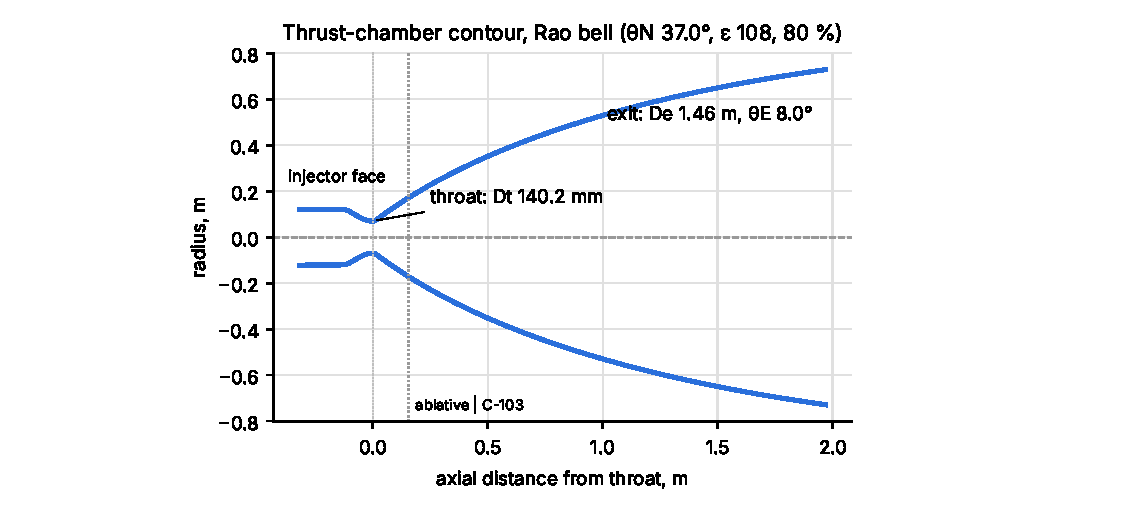
\includegraphics[width=0.95\textwidth]{fig_contour.pdf}
\caption{Thrust-chamber contour from the injector face to the nozzle exit.}\label{fig:contour}\end{figure}

\section{Thermal Design}\label{sec:thermal}
The gas-side heat-transfer coefficient follows Bartz [3; 1, Eq.~4-13]; at the throat $h_g = 2{,}286$~W/(m$^2$K).
The 3{,}042~K core gas is kept off the wall by running the injector's outer ring fuel-rich: 12.5~\% of the flow at
O/F 0.60 (1{,}541~K gas), with the core at O/F 1.92. This is the smallest ring flow that keeps the throat surface below
the 1{,}900~K wear onset of silica phenolic with the heat flux increased by 30~\%; it costs 0.78~s of $I_{sp}$. The
throat heat flux with the ring is 3.1~MW/m$^2$ into a 700~K wall (Fig.~\ref{fig:q}).

The chamber and throat are lined with tape-wrapped silica phenolic to area ratio 6. Silica phenolic was chosen over
carbon phenolic because it resists oxidation by the H$_2$O and CO$_2$ in NTO/MMH exhaust and insulates better. Beyond
area ratio 6 the wall is a radiation-cooled C-103 niobium skirt with an R512E silicide coating. An insulating ring
between the liner and the injector limits soak-back after the longest burn. Results are in Table~\ref{tab:cool} and
Figs.~\ref{fig:wall}--\ref{fig:char}. The liner life is an analytical prediction based on assumed ablator properties
and the Bartz estimate. It requires material characterization and hot-fire testing.

\begin{table}[H]\centering\small\caption{Thermal design results (bounding case: heat flux $\times$ 1.3).}\label{tab:cool}
\begin{tabular}{lp{9.4cm}}\toprule
Item & Value \\\midrule
Liner extent & injector face to area ratio 6 (0.474~m) \\
Liner thickness / mass & 82.6~mm / 66.4~kg \\
Design firing time & 3{,}305~s (1.25 $\times$ 2{,}644~s cumulative) \\
Throat surface temperature & 1{,}806~K (wear onset 1{,}900~K); throat recession 0 \\
Maximum recession & 1.38~mm at 146~mm downstream of the throat (area ratio 5.8) \\
Char depth at end of life & 50.9~mm \\
Titanium case temperature at end of life & 354~K (bond-line limit 420~K) \\
C-103 extension peak temperature & 1{,}389~K nominal, 1{,}477~K bounding (limit 1{,}600~K) \\
Injector after the longest burn (1{,}250~s) & 399~K with insulating ring (MMH boils at 442~K at 1~MPa); about 505~K without \\
\bottomrule\end{tabular}\end{table}
\begin{figure}[H]\centering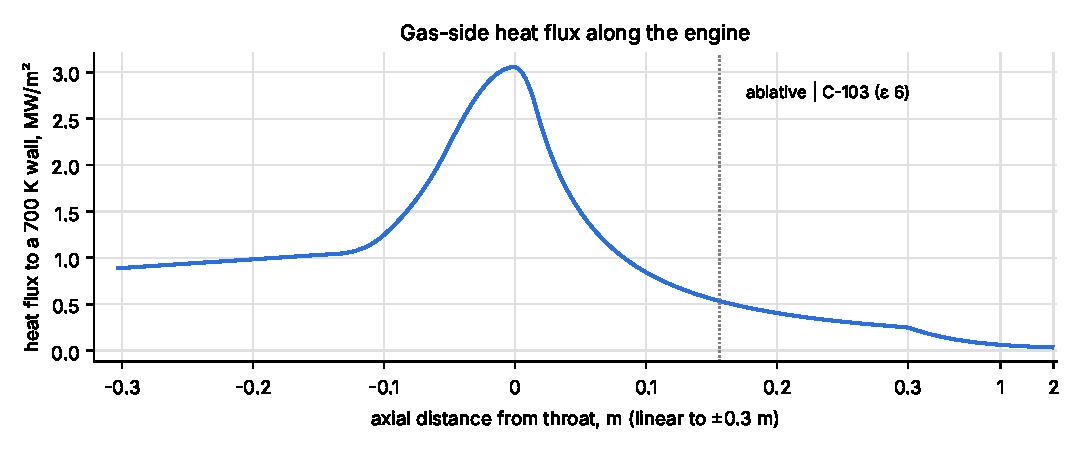
\includegraphics[width=0.92\textwidth]{fig_heatflux.pdf}
\caption{Gas-side heat flux along the engine.}\label{fig:q}\end{figure}
\begin{figure}[H]\centering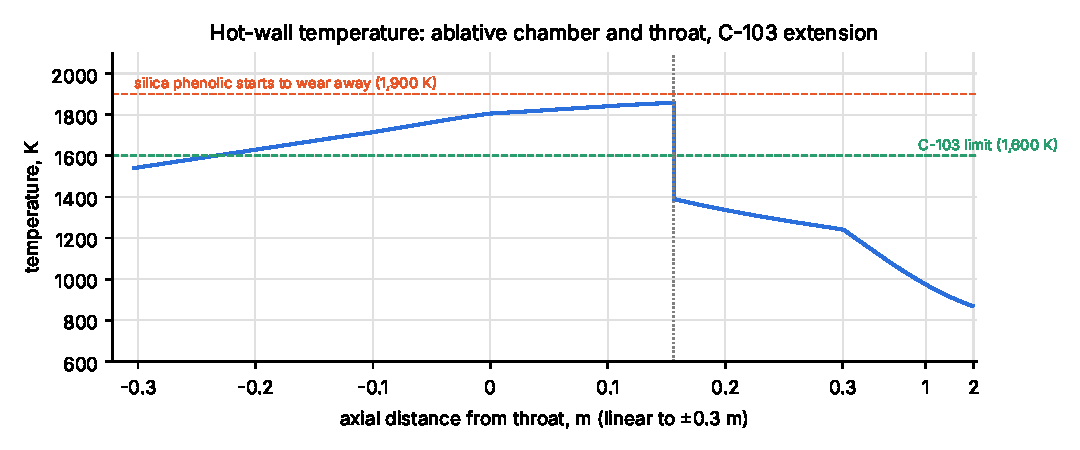
\includegraphics[width=0.92\textwidth]{fig_walltemp.pdf}
\caption{Hot-wall temperature: silica-phenolic liner (left of the dotted line) and C-103 extension.}\label{fig:wall}\end{figure}
\begin{figure}[H]\centering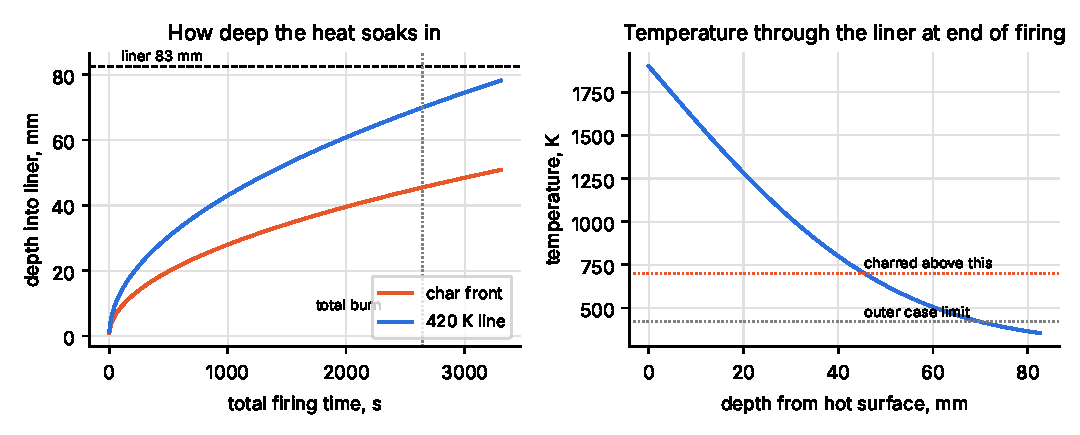
\includegraphics[width=0.92\textwidth]{fig_char.pdf}
\caption{Silica-phenolic liner temperature through the wall at the throat.}\label{fig:char}\end{figure}

\textbf{Nozzle extension wall.} The C-103 wall is 0.6~mm thick. Internal pressure is 19.9~kPa at the attach station
(Mach 3.0) and 0.44~kPa at the exit, so the hoop stress is at most 5.7~MPa, far below the strength of C-103 at
1{,}389~K. A radiation-cooled wall runs at radiation equilibrium whatever its thickness, so thickness does not affect
temperature. The governing loads are stiffness, vibration, gimbal and handling loads, and the attach flange. These are
covered only by a 25~\% mass allowance for stiffening rings, flange and coating, so the extension structure is
preliminary until checked against the mechanical load cases.

\section{Injector}
Unlike-doublet NTO--MMH elements are used. The NTO orifices take 20~\% of the injector-end pressure; the MMH orifices
are sized for best mixing by Rupe's criterion $\rho_o V_o^2 d_o = \rho_f V_f^2 d_f$, giving 26~\%. Both exceed 15~\%,
which decouples the feed system from the combustion. The element flows sum to the engine totals
(Table~\ref{tab:inj}).
\begin{table}[H]\centering\small\caption{Injector design and flow balance.}\label{tab:inj}
\begin{tabular}{lrrr}\toprule
Parameter & Core & Outer ring & Total \\\midrule
Elements & 120 & 48 & 168 \\
NTO / MMH per element, g/s & 38.11 / 19.81 & 7.76 / 12.93 & -- \\
NTO / MMH flow, kg/s & 4.574 / 2.377 & 0.372 / 0.621 & 4.946 / 2.998 \\
Flow fraction / O/F & 87.5~\% / 1.92 & 12.5~\% / 0.60 & 100~\% / 1.65 \\
Orifice diameter NTO / MMH, mm & 1.753 / 1.338 & 0.791 / 1.081 & -- \\
Jet velocity NTO / MMH, m/s & 15.7 / 23.0 & 15.7 / 15.6 & -- \\
$\Delta P$ / injector-end pressure, NTO / MMH & 20~\% / 26~\% & shared manifolds & -- \\
\bottomrule\end{tabular}\end{table}
\begin{table}[H]\centering\small\caption{Acoustic modes and cavities.}\label{tab:acoustic}
\begin{tabular}{lr}\toprule
Quantity & Value \\\midrule
Chamber sound speed, m/s & 1{,}236 \\
1T / 1R / 1L frequency, Hz & 2{,}984 / 6{,}210 / 1{,}947 \\
Quarter-wave cavities (tuned to 1T), number / depth & 12 / 59.4~mm \\
Injector mass (304L), kg & 10.0 \\
\bottomrule\end{tabular}\end{table}

\section{Feed and Pressurization System}
\subsection{Pressure ladder}
Pressures are referenced as follows:
\begin{itemize}
\item \textbf{Chamber pressure:} $P_c = 0.862$~MPa, the nozzle-entrance stagnation pressure.
\item \textbf{Injector-end pressure:} 0.8827~MPa, which is $P_c$ plus the Rayleigh loss.
\item \textbf{Injector orifice drops:} referenced to the injector-end pressure.
\end{itemize}
Each component loss is added from the chamber back to the tank, separately for each propellant (Table~\ref{tab:ladder},
Fig.~\ref{fig:ladder}). Both tanks run at one regulated ullage pressure, 1.279~MPa; trim orifices absorb the difference
between the two sides. The tank maximum expected operating pressure (MEOP) is 1.15 times the ullage pressure,
1.47~MPa, set by the relief-valve crack pressure (1.10 times) plus tolerance.

\begin{table}[H]\centering\small\caption{Pressure ladder at the design point, MPa (upstream pressure of each element).}\label{tab:ladder}
\begin{tabular}{lrr}\toprule
Station & NTO & MMH \\\midrule
Chamber, nozzle-entrance stagnation & 0.862 & 0.862 \\
Injector end (chamber side of the injector face) & 0.883 & 0.883 \\
Injector manifold (orifice $\Delta P$ 177 / 231~kPa) & 1.059 & 1.114 \\
Engine valve inlet ($\Delta P$ 40~kPa) & 1.099 & 1.154 \\
Trim orifice inlet ($\Delta P$ 60 / 20~kPa) & 1.160 & 1.174 \\
Filter inlet ($\Delta P$ 20~kPa) & 1.180 & 1.194 \\
Gimbal flex line inlet ($\Delta P$ 15~kPa) & 1.195 & 1.209 \\
Feed line inlet (line $\Delta P$ 64 / 50~kPa) & 1.259 & 1.259 \\
Latch valve inlet ($\Delta P$ 15~kPa) & 1.274 & 1.274 \\
Tank outlet / PMD ($\Delta P$ 5~kPa) = tank ullage & 1.279 & 1.279 \\
\midrule
Helium regulator outlet & \multicolumn{2}{c}{1.329} \\
Tank MEOP / relief crack & \multicolumn{2}{c}{1.47 / 1.41} \\
Minimum usable helium bottle pressure (regulator dropout) & \multicolumn{2}{c}{2.33} \\
\bottomrule\end{tabular}\end{table}
\begin{figure}[H]\centering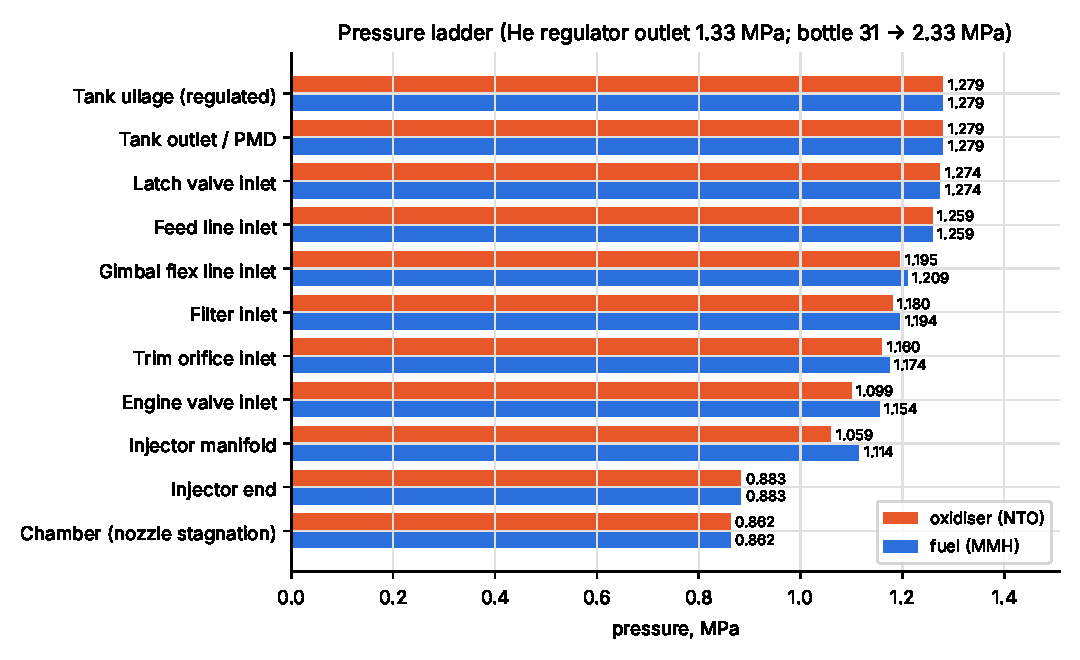
\includegraphics[width=0.9\textwidth]{fig_ladder.pdf}
\caption{Pressure ladder at the design point.}\label{fig:ladder}\end{figure}

\subsection{Feed lines and valve-closure surge}
Both feed lines are 1.5~in $\times$ 0.065~in 321 stainless tube, sized for at most 4~m/s (Table~\ref{tab:lines}). On
engine shutdown the valves close in 50~ms, longer than the pressure-wave round trip, so the surge is reduced below the
instantaneous (Joukowsky) value. The surge is a pressure increase at the closing valve. The tank ullage is held at
constant gas pressure, so the wave is relieved at the tank outlet and the tanks do not see it. The components between
the tank outlet and the engine valve are therefore rated to a line design pressure of 2.2~MPa, which is the tank MEOP
plus the larger surge. At that pressure the tube hoop stress is 23~MPa against 205~MPa yield, a factor of 9.0.

\begin{table}[H]\centering\small\caption{Feed lines.}\label{tab:lines}
\begin{tabular}{lrr}\toprule
Parameter & NTO & MMH \\\midrule
Routed length (CAD), m & 0.5 & 5.6 \\
Tube OD $\times$ wall, in & 1.5 $\times$ 0.065 & 1.5 $\times$ 0.065 \\
Velocity, m/s & 3.6 & 3.6 \\
Line and fittings $\Delta P$, kPa & 64 & 50 \\
Surge increment at 50~ms closure, MPa & 0.42 & 0.69 \\
Peak pressure at the engine valve (valve inlet + surge), MPa & 1.52 & 1.85 \\
Line design pressure (MEOP + largest surge), MPa & \multicolumn{2}{c}{2.2} \\
\bottomrule\end{tabular}\end{table}
The NTO pressure drop was computed for an assumed 2~m line and is conservative for the 0.5~m routed length.

\subsection{Propellant tanks}
Each tank holds the full propellant load at the specified density plus 5~\% ullage (3~\% gas space and 2~\% liquid
expansion from 293 to 305~K) and 0.5~\% PMD displacement. Wall thickness uses a burst factor of 2.0 on the 1.47~MPa
MEOP. Shell mass is the membrane mass $\times$ 1.30 for welds, bosses, girth ring and mounts (Table~\ref{tab:tanks}).
\begin{table}[H]\centering\small\caption{Propellant tanks (baseline used in the analysis and the CAD).}\label{tab:tanks}
\begin{tabular}{lrr}\toprule
Parameter & NTO (lower) & MMH (upper) \\\midrule
Propellant mass, kg & 13{,}075 & 7{,}925 \\
Propellant volume at 293~K, m$^3$ & 9.080 & 9.057 \\
Tank volume, m$^3$ & 9.580 & 9.555 \\
Inner diameter, m & 2.635 & 2.633 \\
Wall (Ti-6Al-4V), mm & 2.16 & 2.16 \\
MEOP, MPa & 1.47 & 1.47 \\
Free gas volume at 283 / 293 / 305~K, \% of tank & 6.2 / 4.8 / 2.9 & 6.2 / 5.2 / 3.9 \\
Shell (membrane 209.5 / 209.0~kg $\times$ 1.30) / PMD mass, kg & 272 / 15 & 271 / 15 \\
\bottomrule\end{tabular}\end{table}

\subsection{Helium pressurization}
At end of burn both tanks are full of helium at 1.279~MPa (19.1~m$^3$). The required helium is computed for the cold
design case, 273~K with adiabatic bottle expansion, using real-gas compressibility in the bottles. A 10~\% margin is
added for leakage and pre-pressurization (Table~\ref{tab:he}). The stored 86.5~kg is the initial inventory. At 31~MPa
and 273~K the compressibility factor is $Z = 1.16$, so 86.5~kg occupies 1.838~m$^3$; an ideal-gas estimate would put
100~kg in the same volume. A time-stepped blowdown of the bottles (adiabatic, 273~K start, tanks held at 1.279~MPa)
ends at 5.96~MPa, above the 2.33~MPa regulator dropout, with 31.3~kg left in the bottles (Fig.~\ref{fig:he}).
\begin{table}[H]\centering\small\caption{Helium system.}\label{tab:he}
\begin{tabular}{lp{7.6cm}}\toprule
Item & Value \\\midrule
Required, isothermal / adiabatic bottles, 273~K, kg & 47.2 / 78.6 \\
Initial inventory (adiabatic 273~K + 10~\%), kg & 86.5 \\
Bottles & 4 COPVs, 0.460~m$^3$ each (1.838~m$^3$), 0.957~m diameter, 31~MPa \\
Bottle mass (all four), kg & 380 \\
Bottle pressure at end of burn (simulated) & 5.96~MPa (dropout 2.33~MPa) \\
Helium delivered / remaining, kg & 55.2 / 31.3 \\
\bottomrule\end{tabular}\end{table}
\begin{figure}[H]\centering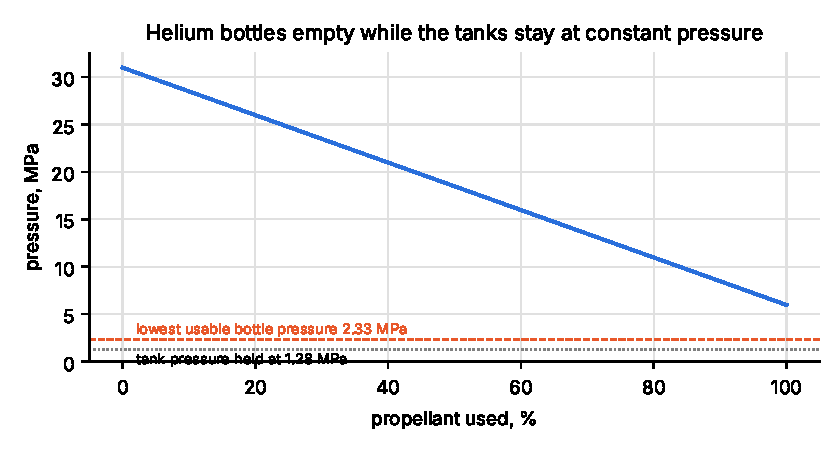
\includegraphics[width=0.62\textwidth]{fig_helium.pdf}
\caption{Helium bottle pressure as the propellant is used (design case).}\label{fig:he}\end{figure}

\section{Materials}
\begin{table}[H]\centering\small\caption{Materials and margins (allowables assumed, to be verified).}\label{tab:mat}
\adjustbox{max width=\linewidth}{\begin{tabular}{p{2.6cm}p{2.6cm}p{3.7cm}p{3.3cm}p{2.3cm}}\toprule
Part & Material & Operating condition & Allowable & Margin \\\midrule
Propellant tanks & Ti-6Al-4V & 448~MPa membrane stress at MEOP & 895~MPa ultimate & factor 2.00 (2.0 required) \\
Chamber/throat liner & silica phenolic & 1{,}806~K surface & 1{,}900~K wear onset & 94~K \\
Liner back face / case & Ti-6Al-4V & 354~K; 108~MPa & 420~K bond line; 828~MPa yield & 66~K; factor 7.7 \\
Nozzle extension & C-103 + R512E & 1{,}389~K & 1{,}600~K & 211~K \\
Injector & 304L & 399~K after shutdown & 442~K (MMH boiling at 1~MPa) & 43~K \\
Feed lines & 321 stainless & 2.2~MPa design pressure; 23~MPa hoop stress & 205~MPa yield & factor 9.0 \\
Helium bottles & COPV (Ti liner, carbon overwrap) & 31~MPa & burst $\geq$ 1.5 $\times$ MEOP (vendor) & vendor item \\
Seals, valve seats & PTFE / PCTFE & 283--305~K, NTO and MMH & 73--533~K (PTFE) & large \\
\bottomrule\end{tabular}}\end{table}
NTO must be procured to MIL-PRF-26539 with controlled nitric-oxide content to avoid stress-corrosion cracking of the
titanium tanks.

\section{Mass Budget}
The line mass uses the routed CAD lengths (Sec.~\ref{sec:cad}), 2.5~kg more than the original allowance.
\begin{table}[H]\centering\small\caption{Propulsion-system mass budget.}\label{tab:mass}
\begin{tabular}{lr|lr}\toprule
Engine & kg & Feed and pressurization & kg \\\midrule
Injector & 10.0 & NTO tank & 271.9 \\
Valves & 14.0 & MMH tank & 271.2 \\
Liner & 66.4 & PMDs & 30.0 \\
Case & 10.0 & COPVs & 379.9 \\
Extension (32.5 bare $\times$ 1.25) & 40.7 & Helium & 86.5 \\
Gimbal actuators & 20.0 & Components (Table~\ref{tab:comp}) & 40.0 \\
Miscellaneous & 10.0 & Lines (CAD) & 15.4 \\
 & & Supports & 109.3 \\\midrule
\textbf{Engine} & \textbf{171.1} & \textbf{Feed and pressurization} & \textbf{1{,}204.3} \\\midrule
\multicolumn{4}{l}{\textbf{Propulsion system: 1{,}375~kg, 21.2~\% of the 6{,}500~kg structural mass}} \\
\bottomrule\end{tabular}\end{table}
\begin{table}[H]\centering\small\caption{Components allowance (allocated, to be replaced by vendor data).}\label{tab:comp}
\begin{tabular}{lrl}\toprule
Item & kg & In CAD \\\midrule
Helium regulators (2, in series) & 6 & regulator panel \\
Helium check valves (2) & 4 & regulator panel \\
Helium latch / isolation valves (2), fill valve, filter & 7 & budget only \\
Relief valves (2) & 3 & budget only \\
Propellant latch valves (2) & 10 & budget only \\
Propellant filters (2) & 3 & budget only \\
Propellant fill, drain and vent valves (4) & 4 & budget only \\
Transducers and fittings & 3 & budget only \\\midrule
\textbf{Total} & \textbf{40} & panel = 10~kg \\
\bottomrule\end{tabular}\end{table}

\section{CAD Model}\label{sec:cad}
The propulsion bay is modelled in Onshape as one parametric FeatureScript feature, generated directly from the analysis
outputs (engine contour and layout). It contains:
\begin{itemize}
\item the engine: liner, case and C-103 extension as smooth bodies of revolution, the injector plate with 12 acoustic
cavities, and the head, valve and gimbal stack;
\item both tanks and the four COPVs;
\item the feed and helium lines, and the regulator panel;
\item reference shells for the SM, the capsule and the launch escape system (LES), traced from the PDR drawing [6].
\end{itemize}
A \emph{Cut view} option removes the $-Y$ half of every body (Figs.~\ref{fig:cutfront}--\ref{fig:cutengine}). Units
are millimetres; the origin is at the SM base on the axis, with $+Z$ up. Lumped items (head stack, COPVs, regulator
panel) carry their budget masses. The acoustic cavities are modelled as \O16~mm bores on a 100~mm pitch radius.

\begin{figure}[H]\centering
\begin{minipage}{0.48\textwidth}\centering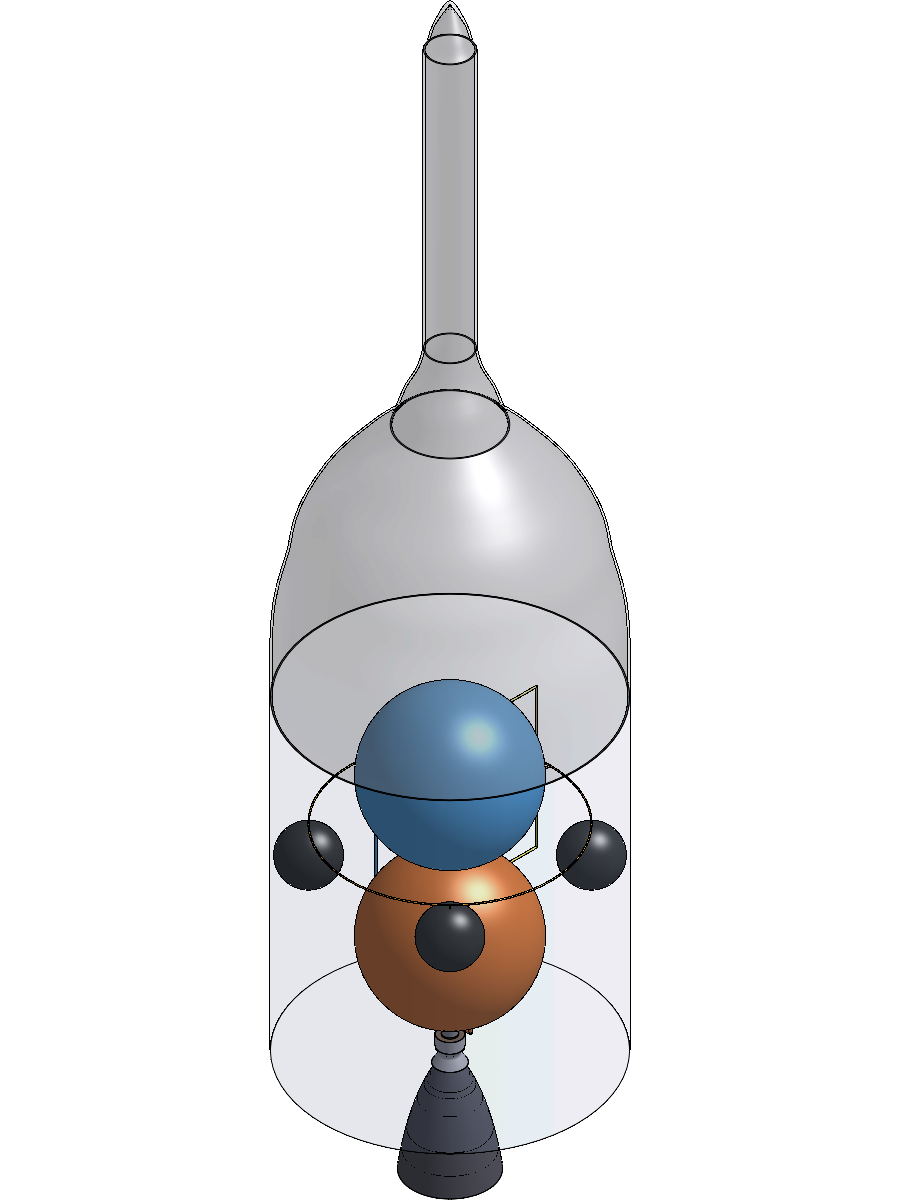
\includegraphics[width=\textwidth,height=0.36\textheight,keepaspectratio]{cad_iso.png}
\caption{Full model, isometric.}\label{fig:iso}\end{minipage}\hfill
\begin{minipage}{0.48\textwidth}\centering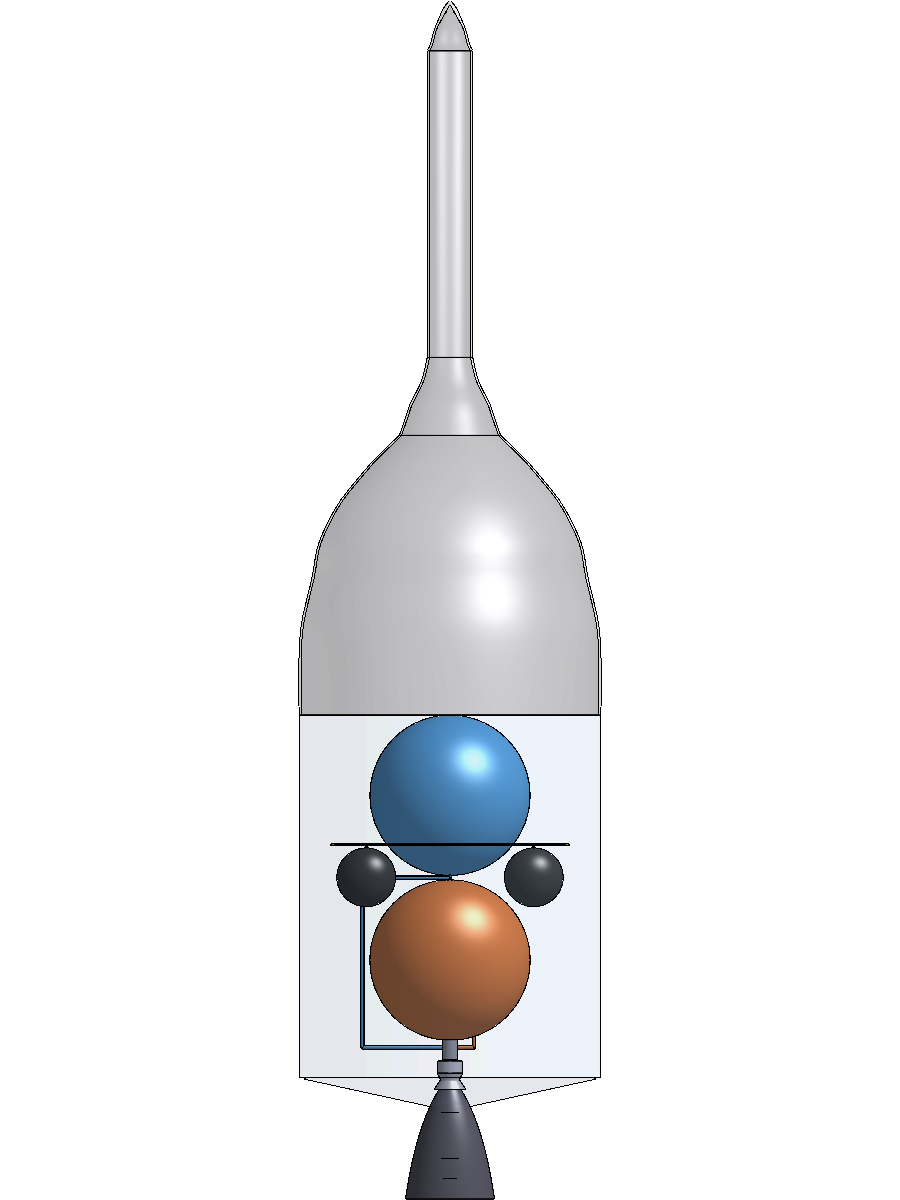
\includegraphics[width=\textwidth,height=0.36\textheight,keepaspectratio]{cad_front.png}
\caption{Full model, front.}\label{fig:front}\end{minipage}
\end{figure}
\begin{figure}[H]\centering
\begin{minipage}{0.48\textwidth}\centering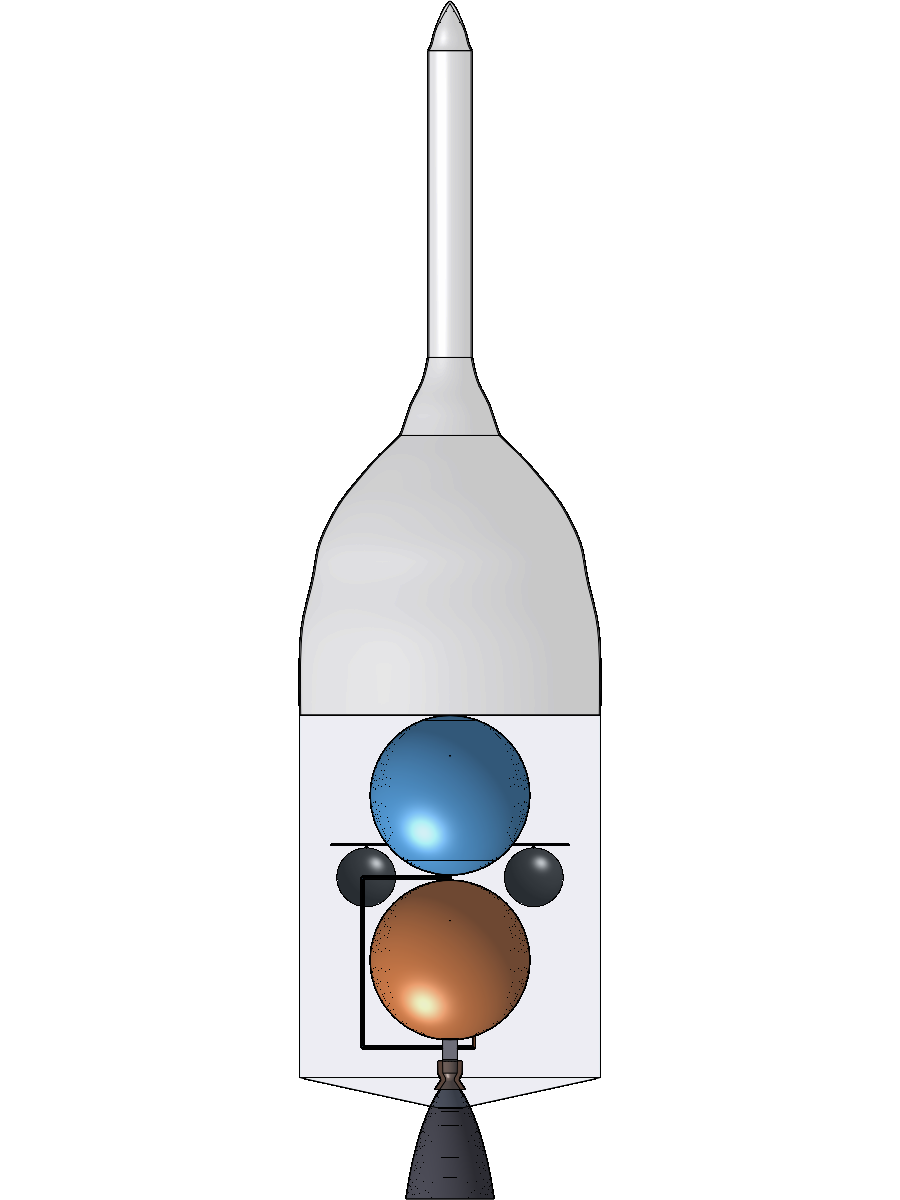
\includegraphics[width=\textwidth,height=0.36\textheight,keepaspectratio]{cad_cut_front.png}
\caption{Cut view, front.}\label{fig:cutfront}\end{minipage}\hfill
\begin{minipage}{0.48\textwidth}\centering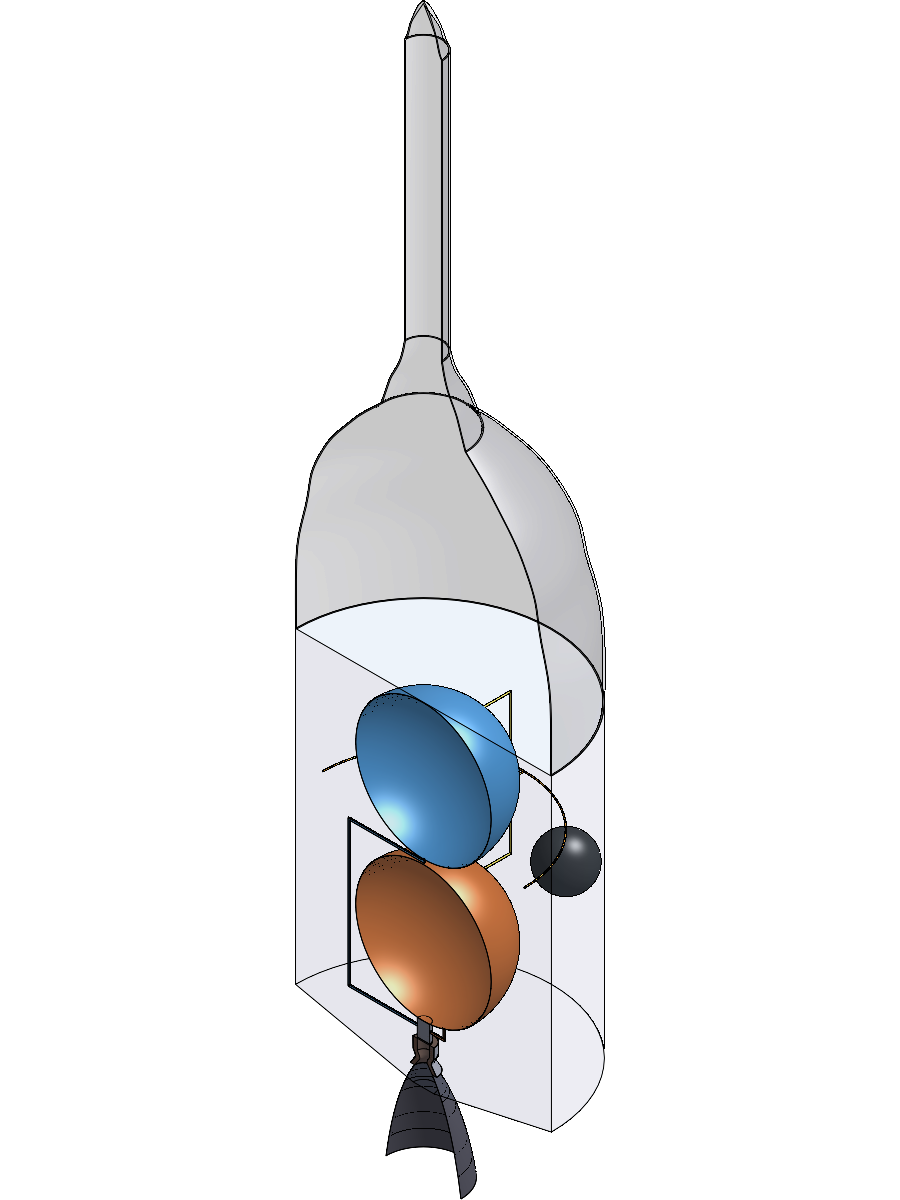
\includegraphics[width=\textwidth,height=0.36\textheight,keepaspectratio]{cad_cut_iso.png}
\caption{Cut view, isometric.}\label{fig:cutiso}\end{minipage}
\end{figure}
\begin{figure}[H]\centering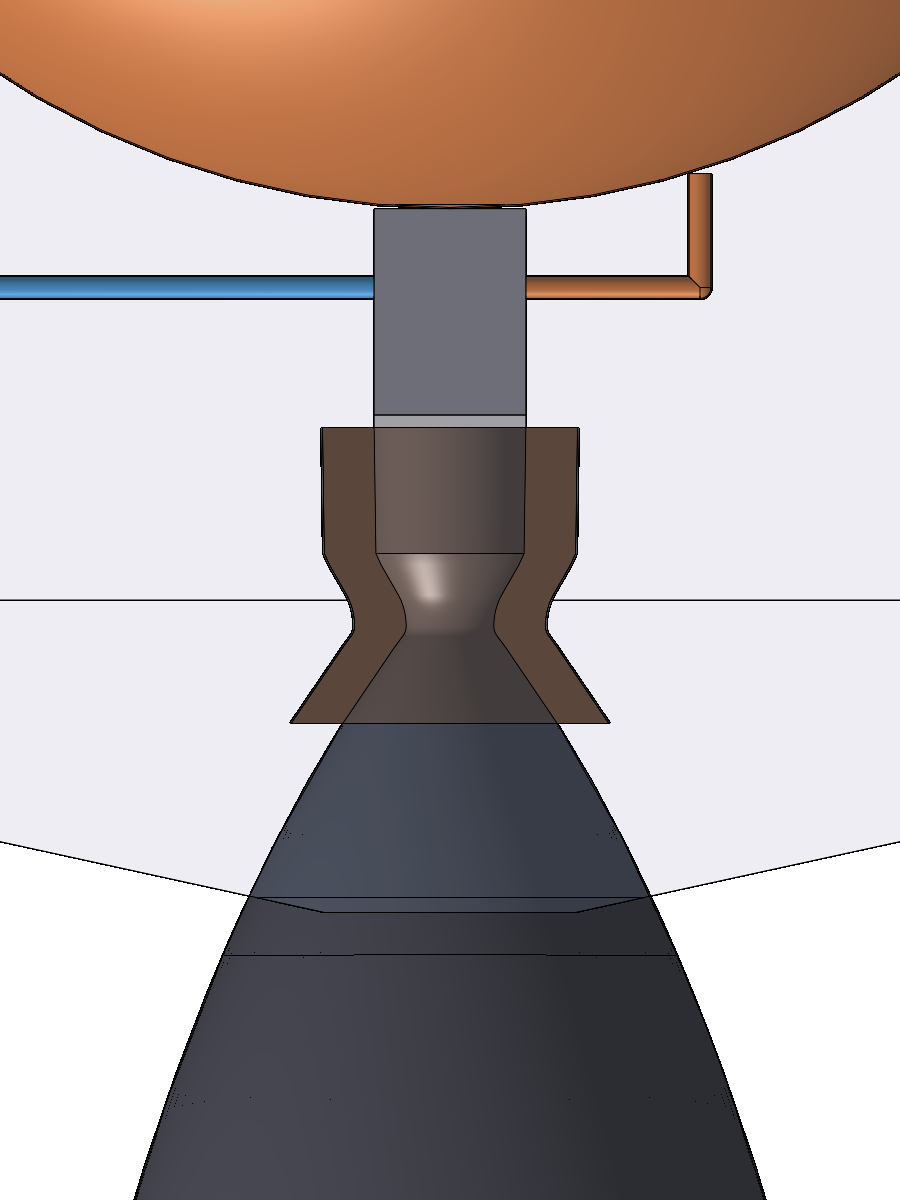
\includegraphics[width=0.55\textwidth,height=0.38\textheight,keepaspectratio]{cad_cut_engine.png}
\caption{Cut view of the engine with the NTO (right) and MMH (left) feed lines entering the valve stack.}\label{fig:cutengine}\end{figure}

\begin{table}[H]\centering\small\caption{Layout and clearances (from the CAD model).}\label{tab:layout}
\begin{tabular}{p{4.6cm}p{11cm}}\toprule
Item & Value \\\midrule
Gimbal plane / injector face / throat / nozzle exit, $z$ & 626 / 276 / $-42$ / $-2{,}010$~mm \\
NTO tank centre; outer diameter & $z = 1{,}946$~mm; 2.639~m \\
MMH tank centre; outer diameter & $z = 4{,}674$~mm; 2.637~m \\
Gap between tanks (MMH line passes through it) & 90~mm (26~mm each side of the line) \\
Tank stack, gimbal plane to MMH top & 5.366~m; top at $z = 5{,}992$~mm, 7.6~mm below the SM top \\
COPVs & 4 at 45/135/225/315$^\circ$, radius 1{,}961~mm, $z = 3{,}315$~mm \\
COPV to SM wall / to tanks & 50~mm / 589~mm (radial space beside the tanks: 1.17~m) \\
Feed line routes & NTO: lower dome to $+X$ side of the valve stack; MMH: bottom pole, tank gap, down at $x = -1{,}450$~mm \\
Helium lines & 0.375~in HP ring ($z = 3{,}854$~mm) to the regulator; 0.75~in LP lines to each upper dome \\
Interference (136 body pairs) & none; connected parts meet within 0--0.12~mm \\
Outside the SM envelope & C-103 extension only (exit 2.01~m below the SM base, by design) \\
\bottomrule\end{tabular}\end{table}

The CAD masses agree with the budget once undrawn items are accounted for:
\begin{itemize}
\item \textbf{Liner:} 66.1~kg in the CAD against 66.4~kg in the budget.
\item \textbf{Bare tank membranes:} 209.5 and 209.0~kg; times 1.30 these match the 272 and 271~kg budget.
\item \textbf{Bare extension wall:} 33.2~kg against 32.5~kg calculated.
\item \textbf{Case:} 6.5~kg; the budget adds 3~kg of flanges.
\item \textbf{Injector plate:} 6.9~kg; the budget adds a 2.6~kg manifold.
\item \textbf{Lines:} 15.4~kg, now carried in the budget.
\end{itemize}

\section{Requirements Compliance}
\begin{table}[H]\centering\small\caption{Design against the Crew Capsule requirements.}\label{tab:comply}
\adjustbox{max width=\linewidth}{\begin{tabular}{lll}\toprule
Requirement & Required & Design (status) \\\midrule
Thrust, engines & 25~kN, 1 & 25~kN vacuum, 1 (met) \\
Specific impulse & $\geq$ 280~s & 320.8~s nominal, 303.5~s pessimistic (met, predicted) \\
$\Delta v$ with $M_0$ 38{,}000~kg, $M_b$ 17{,}000~kg & 2{,}209~m/s & 2{,}531~m/s nominal, 2{,}394~m/s pessimistic (met, predicted) \\
Propellant load & 21{,}000~kg at O/F 1.65 & fits with 2.9~\% free gas volume at the 305~K hot case (met) \\
$T/W$ at the Moon & 0.405 / 0.905 & unchanged (met) \\
Firing life & 2{,}644~s cumulative, 11 starts & liner 3{,}305~s predicted; 22 design starts (preliminary) \\
SM envelope & 6~m section; 2.01~m below base & stack 5.366~m (7.6~mm clearance); engine 2.636~m of 2.642~m (met) \\
Propulsion mass & within 6{,}500~kg $M_s$ & 1{,}375~kg, 21.2~\% (met) \\
\bottomrule\end{tabular}}\end{table}

\section{Conclusions and Open Items}
The 25~kN pressure-fed NTO/MMH engine is predicted to deliver 320.8~s vacuum $I_{sp}$ (303.5~s pessimistic) at 0.862~MPa
chamber pressure, O/F 1.65 and area ratio 108, with an 80~\% Rao bell of 1.457~m exit diameter. A silica-phenolic
chamber protected by a fuel-rich outer ring, followed by a C-103 extension, is predicted to survive the 2{,}644~s
cumulative firing with margin. The tanks, the four helium bottles and the engine fit the PDR SM envelope, and the tanks
hold the full propellant load at the hot case. The propulsion system mass is 1{,}375~kg.

These are analytical results. The following items remain open:
\begin{enumerate}
\item Heat flux, fuel-rich-ring effectiveness and ablator properties are uncalibrated. The liner life must be
confirmed by material characterization and hot-fire tests, including restart thermal cycling.
\item The nozzle-extension structure (wall, attach flange and stiffening rings) must be analysed for vibration, gimbal
and handling loads.
\item The feed-line transient must be confirmed with a system water-hammer model and component ratings of at least
2.2~MPa.
\item Feed lines need flexible sections across the gimbal; the components allowance needs vendor masses.
\item The tank stack leaves 7.6~mm below the SM top; the capsule interface must be checked.
\item NTO must be procured to MIL-PRF-26539 with controlled nitric-oxide content.
\end{enumerate}

\begin{thebibliography}{99}\small
\bibitem{hh} Huzel, D. K. and Huang, D. H., \emph{Modern Engineering for Design of Liquid-Propellant Rocket Engines}, AIAA Progress in Astronautics and Aeronautics Vol. 147, 1992.
\bibitem{cea} Gordon, S. and McBride, B. J., \emph{Computer Program for Calculation of Complex Chemical Equilibrium Compositions and Applications}, NASA RP-1311, 1994.
\bibitem{bartz} Bartz, D. R., ``A Simple Equation for Rapid Estimation of Rocket Nozzle Convective Heat Transfer Coefficients,'' \emph{Jet Propulsion}, Vol. 27, No. 1, 1957, pp. 49--51.
\bibitem{rao} Rao, G. V. R., ``Exhaust Nozzle Contour for Optimum Thrust,'' \emph{Jet Propulsion}, Vol. 28, No. 6, 1958, pp. 377--382.
\bibitem{abeona} Project ABEONA, \texttt{Mission\_Breakdown.xlsx} (Crew Capsule tab) and \emph{Preliminary Design Report}, 2026.
\bibitem{pdrr} Kempf, A., Bratt, E., LeRoy, M., Bernal, R., Wiser, S., and Rouland, S., ``Preliminary Design Review, Project ABEONA,'' class presentation, slide 7 (Crew Capsule), 2026.
\bibitem{rcea} Taylor, C., \emph{RocketCEA}, version 1.2.3, rocketcea.readthedocs.io.
\bibitem{rp} Taylor, C., \emph{RocketProps}, rocketprops.readthedocs.io.
\bibitem{belair} Belair, M. et al., ``Artemis I Engine Performance,'' NTRS 20240003648, 2024.
\bibitem{bert} Bertolino, J. D. and Boyd, W. C., ``Uprated OMS Engine Status -- Sea Level Testing Results,'' NTRS 19910014943, 1990.
\bibitem{nasacea} NASA Glenn Research Center, CEA thermodynamic database \texttt{thermo.inp}, github.com/nasa/cea.
\bibitem{zh} Zucrow, M. J. and Hoffman, J. D., \emph{Gas Dynamics}, Vol. 2, Wiley, 1977.
\end{thebibliography}
\end{document}
